\documentclass[12pt,a4paper]{article}

% Кодування/мови — в такому порядку
\usepackage[utf8]{inputenc}
\usepackage[T2A]{fontenc}
\usepackage[ukrainian]{babel}
\usepackage{cmap}

\usepackage{geometry}
\geometry{left=2cm,right=2cm,top=2cm,bottom=2cm}

\usepackage{graphicx}
\usepackage{array,multirow,booktabs,makecell}
\usepackage{caption}
\renewcommand{\thetable}{\arabic{table}}
\usepackage[table]{xcolor} % <-- це дає \rowcolor і \cellcolor
\captionsetup[table]{name=Таблиця}

\usepackage{amsmath}
\usepackage{pdflscape}
\usepackage{xcolor}

\newcommand{\g}{\cellcolor{gray!25}} % коротке позначення сірого

% Гіперпосилання — тримай наприкінці пакетів, з unicode
\usepackage[unicode]{hyperref}

\renewcommand\cellalign{tc}
\renewcommand\theadalign{cc}
\newcommand{\addh}{\rule{0pt}{3.8ex}} % ДОДАТКОВА ВИСОТА РЯДКА (лише де потрібно)
\renewcommand{\arraystretch}{1.25}

\begin{document}

    \begin{titlepage}

        % Картинка шапки (по центру, з відступом від верху)
        \begin{center}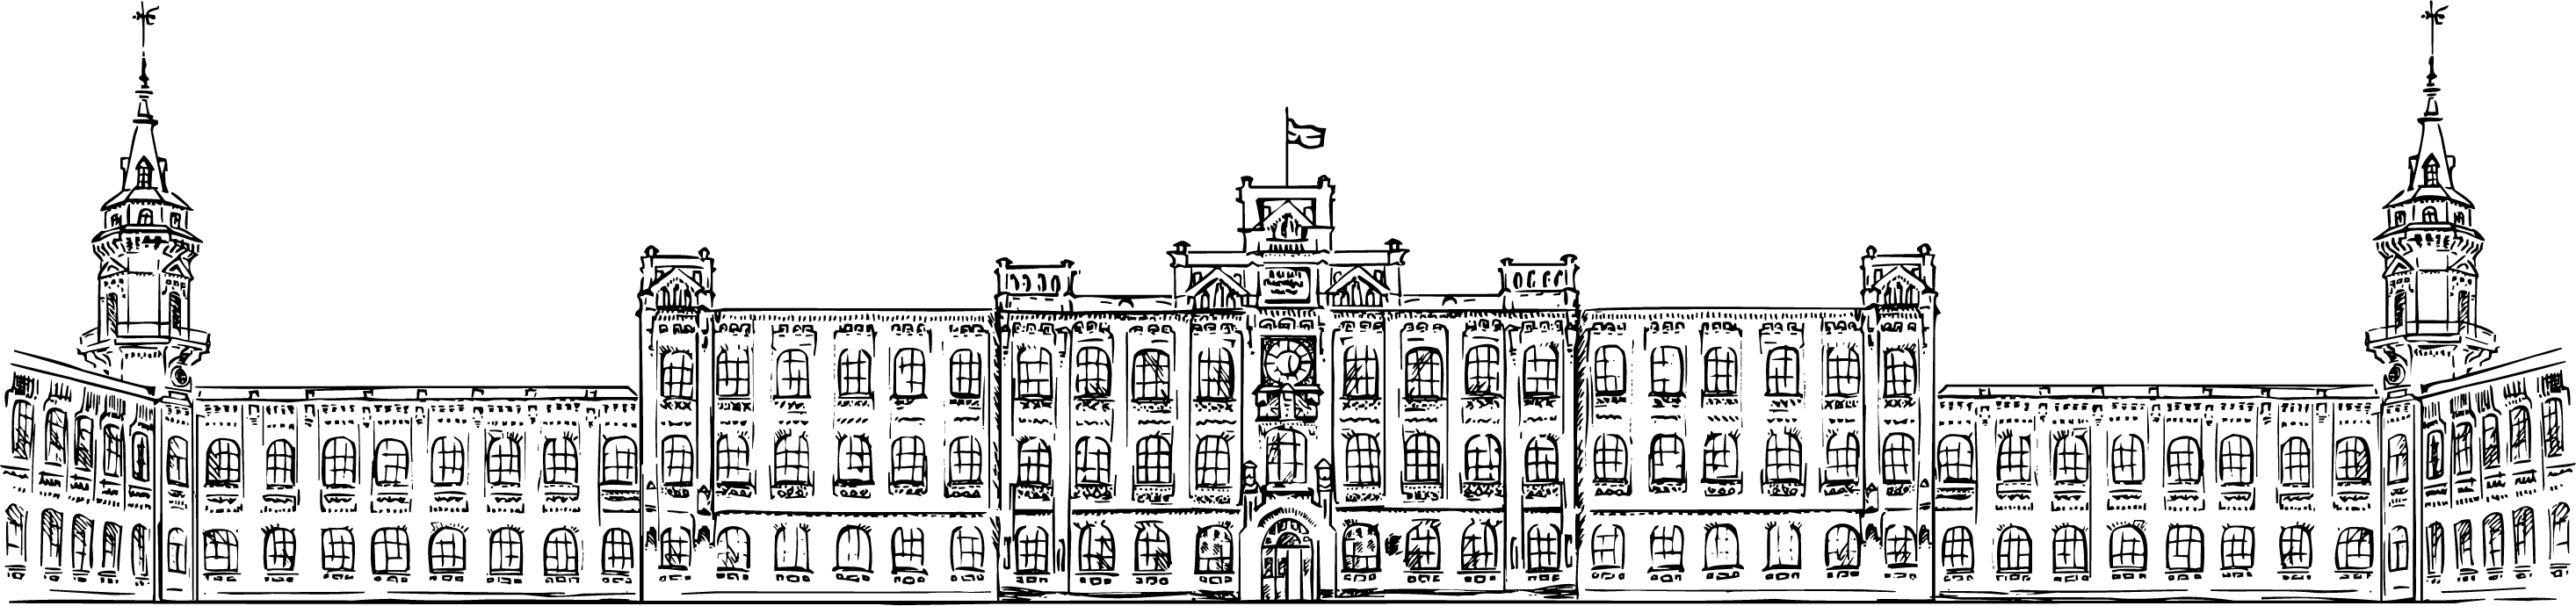
\includegraphics[width=0.7\textwidth]{../../../TITLES/letterhead.png}\end{center}

        \begin{center}
            \large Національний технічний університет України\\
            «Київський політехнічний інститут імені Ігоря Сікорського»\\[1em]
            Факультет інформатики та обчислювальної техніки\\
            Кафедра обчислювальної техніки
        \end{center}

        \vfill

        \begin{center}
            \textbf{\LARGE Теорія електричних кіл та сигналів}\\[2em]
            \textbf{\Large Лабораторна робота №6}\\[0.5em]
            «Дослідження перехідних процесів у лінійних електричних колах з послідовним з'єднанням RC елементів»
        \end{center}

        \vfill

        \begin{flushright}
            Виконав: студент 2 курсу ФІОТ, гр. ІО-41\\
            \textit{Давидчук А.~М.}\\[1em]
            Перевірив: \textit{Лободзинський В.~Ю.}
        \end{flushright}

        \vfill

        \begin{center}Київ --- 2025\end{center}

    \end{titlepage}

    \noindent
    \textbf{\underline{Тема:}} «Дослідження перехідних процесів у лінійних електричних колах з послідовним з'єднанням RC елементів».

    \vspace{1em}

    \noindent
    \textbf{\underline{Мета:}} Дослідження перехідних процесів в електричних колах постійного струму при
послідовному з’єднанні резистивно-ємнісних (RС) елементів

    \begin{center} \textbf{\Large Практична частина} \end{center}

    Усі розрахунки було проведено за допомогою мови програмування Python (вихідний код додано разом із звітом).

    \vspace{1em}

    Моя група: IО-41, мiй порядковий номер у групi: 6. Звiдси $N = 6, S = 1$.

    Загальна структурна схема електричного кола:

    \begin{figure}[h!]
        \renewcommand{\thefigure}{\arabic{figure}} % робимо "3.1", "3.2" і т.д.
        \centering
        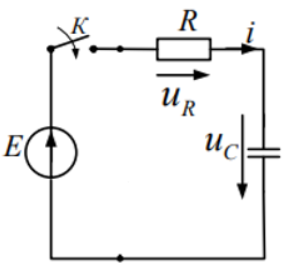
\includegraphics[width=0.5\textwidth]{s0.png}
        \caption{структурна схема електричного кола}
    \end{figure}

    \vspace{1em}

    Розраховані параметри елементів:

    \begin{table}[h!]
        \centering
        \begin{tabular}{|c|c|c|}
            \hline
            $E,\,\text{В}$ & $R,\,\text{Ом}$ & $C,\,\text{Ф}$ \\
            \hline
            11& 16 & $88\cdot10^{-6}$ \\
            \hline
        \end{tabular}
        \caption{Розраховані параметри елементів кола}
    \end{table}

    Розрахована постійна часу $\tau$ та перехідного процесу $T_{\text{пп}}$:

    \begin{table}[h!]
        \centering
        \begin{tabular}{|c|c|}
            \hline
            $\tau,\,\text{с}$ & $T_{\text{пп}},\,\text{с}$ \\
            \hline
            0{,}001408& 0{,}01408 \\
            \hline
        \end{tabular}
        \caption{Розрахована постійна часу та перехідного процесу}
    \end{table}

    На основі $T_{\text{пп}}$, розрахую частоту джерела напруги тактової частоти (генератор прямокутних хвиль):

    \[
    f = T_{\text{пп}}^{-1} \approx 72 \text{ Гц}
    \]

    \newpage

    На основі загальної структури електричного кола та попередньо розрахованих параметрів її елементів, побудую електричну схему у програмі Multisim:

    \begin{figure}[h!]
        \renewcommand{\thefigure}{\arabic{figure}} % робимо "3.1", "3.2" і т.д.
        \centering
        \includegraphics[width=1\textwidth]{scheme.pdf}
        \caption{Електрична схема у програмi Multisim}
    \end{figure}

    \noindent
    Отримуємо осцилограми $u_R(t), u_C(t)$:

    \begin{figure}[h!]
        \renewcommand{\thefigure}{\arabic{figure}} % робимо "3.1", "3.2" і т.д.
        \centering
        
\includegraphics[width=1\textwidth]{graph0.png}
        \caption{Осцилограми напруг на резисторі та на конденсаторі}
    \end{figure}

    \newpage

    Далі визначимо графічно значення $\tau$ при замиканні/розмиканні ключа (використовуватимемо графік $u_C(t)$):

    \begin{figure}[h!]
        \renewcommand{\thefigure}{\arabic{figure}} % робимо "3.1", "3.2" і т.д.
        \centering
        
\includegraphics[width=0.95\textwidth]{graph1.png}
        \caption{Значення $\tau = dx = x_2 - x_1$ при замиканні ключа}
    \end{figure}

    \begin{figure}[h!]
        \renewcommand{\thefigure}{\arabic{figure}} % робимо "3.1", "3.2" і т.д.
        \centering
        
\includegraphics[width=0.95\textwidth]{graph2.png}
        \caption{Значення $\tau = dx = x_2 - x_1$ при розмиканні ключа}
    \end{figure}

    \newpage

    Результати графічного обчислення $\tau$ зведемо до таблиці:

    \begin{table}[h!]
        \centering
        \begin{tabular}{|p{7cm}|p{7cm}|}
            \hline
            \centering $\tau$ при розмиканні ключа, с & \centering $\tau$ при замиканні ключа, с \tabularnewline
            \hline
            \centering $1,4796 \cdot 10^{-3}$& \centering $1,5312 \cdot 10^{-3}$ \tabularnewline
            \hline
        \end{tabular}
    \end{table}

    Далі будемо використовувати осцилограму $u_C(t)$ задля розрахунку значення складових аналітичних виразів $u_C(t), i_C(t)$ при замиканні та розмиканні ключа.
    Аналітичні вирази $u_C(t), i_C(t)$ при замиканні ключа:

    \[
    u_C(t) = E\left(1 - e^{-\dfrac{t}{RC}}\right);
    \]

    \[
    i(t) = \frac{E}{R} e^{-\dfrac{t}{RC}} .
    \]

    Звідси $E = 11$ В, $R = 16$ Ом, $RC = \tau = 1,4796 \cdot 10^{-3}$ с. Побудую графіки:

    \begin{figure}[h!]
        \renewcommand{\thefigure}{\arabic{figure}}
        \centering
        
\includegraphics[width=0.95\textwidth]{graph3.png}
        \caption{Графік виразів $u_C(t)$ та $i_C(t)$ при замиканні ключа}
    \end{figure}

    \newpage

    Аналітичні вирази $u_C(t), i_C(t)$ при розмиканні ключа:

    \[
    u_C(t) = E e^{-\dfrac{t}{RC}};
    \]

    \[
    i(t) = -\frac{E}{R} e^{-\dfrac{t}{RC}}.
    \]

    Тут все незмінне, окрім $\tau = 1,5312 \cdot 10^{-3}$ с (значення $\tau$ я беру як попередньо графічно визначені значення)

    Побудую графiки:

    \begin{figure}[h!]
        \renewcommand{\thefigure}{\arabic{figure}}
        \centering
        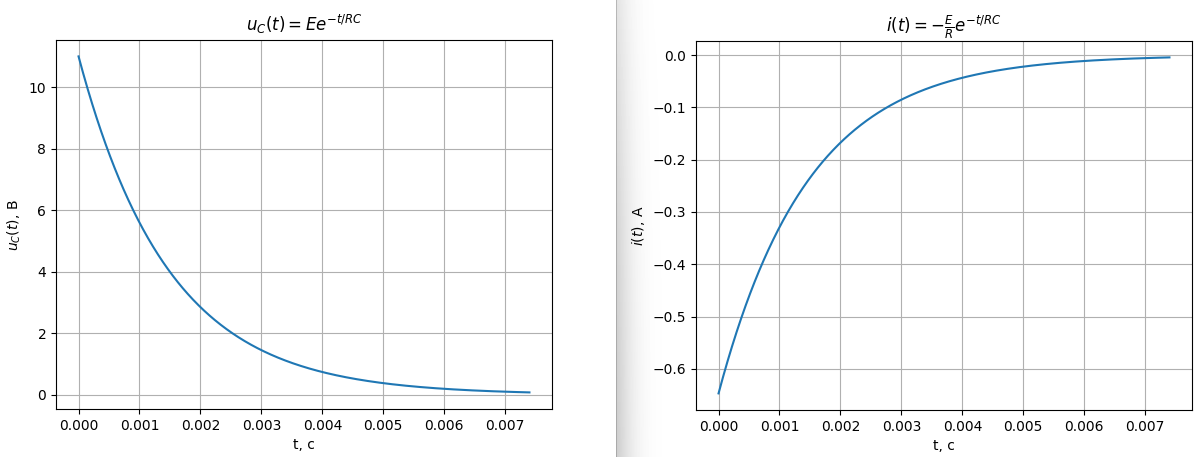
\includegraphics[width=0.95\textwidth]{graph4.png}
        \caption{Графік виразів $u_C(t)$ та $i_C(t)$ при розмиканні ключа}
    \end{figure}

    Також можемо висновувати про закон комутації на основі графіку перехідних процесів, а саме для конденсатора \underline{виконується} закон комутації напруги, згідно з яким
    \[
    u_C(0^-) = u_C(0^+).
    \]

    Це означає, що напруга на конденсаторі не здатна змінюватися миттєво в момент перемикання кола. 
    Ємність накопичує заряд, тому стрибкоподібна зміна напруги потребувала б нескінченно великого струму, що фізично неможливо. 
    З осцилограми видно, що значення $u_C(t)$ безпосередньо перед комутацією та одразу після неї збігаються, 
    тобто напруга залишається безперервною. Отже, закон комутації напруги для конденсатора дотримується.

    \vspace{1em}

    \noindent
    \textbf{\underline{Висновок:}} Постійна часу кола $RC$ визначається як $\tau = RC$, тому опір резистора $R$ безпосередньо впливає 
    на швидкість перехідного процесу. Зі зростанням $R$ збільшується і стала часу $\tau$, унаслідок чого 
    заряджання та розряджання конденсатора відбуваються повільніше: напруга $u_C(t)$ повільніше 
    наближається до усталеного значення, а початковий струм зменшується. 

    Зменшення опору, навпаки, призводить до зменшення $\tau$ та прискорення перехідного процесу. 
    Таким чином, чим більший опір резистора, тим повільніше відбувається перехідний процес у колі $RC$, 
    і чим менший опір, тим швидше система переходить у усталений режим.

\end{document}